\chapter{Konzeption einer graphbasierten Serviceregistry}

Im folgenden Kapitel wird versucht auf Basis der in \vref{chap:Anforderungen} beschriebenen Anforderungen ein Konzept für ein Tool zu erarbeiten, welches als \enquote{intelligente} Service-Registry fungiert. Dazu wird zunächst eine mögliche Technologiewahl erläutert. Danach werden noch einige mögliche Funktionen mithilfe von Beispielen vorgestellt.

\section{Wieso wird ein Graph verwendet?}

Bereits in \citeauthor{Ren2018} wird ein Graph verwendet, um zu beschreiben, wie ein einfacher Übergang zwischen einer ehemals monolithischen Architektur zu einem Microserviceansatz erreicht werden kann. In diesem Fall wird ein Abhängigkeitsgraph verwendet, um die Zusammenhänge zwischen den verschiedenen Komponenten zu beschreiben. Anhand dieses Graphen wird dann versucht, die benötigten Services zu definieren. Der Graph beschreibt also Zusammenhänge zwischen den verschiedenen Services \autocite[Kapitel 3.2 \& Kapitel 3.3]{Ren2018}. Diese Idee bildet auch das Fundament des vorgeschlagenen Konzepts. Um allerdings zu verstehen, wieso ein Abhängigkeitsgraph auch als Basis für eine Serviceregistry dienen kann, muss zuerst erläutert werden, was ein Graph ist und wie Graphdatenbanken dabei helfen können, dieses abstrakte Modell für die Softwareentwicklung nutzbar zu machen.

\begin{definition}[gerichteter Graph]\autocite[Kapitel 1.2]{Bang-Jensen2007}
	Ein gerichteter Graph ist ein geordnetes Tupel $$G = (V,A)$$ für das gilt:
	\begin{itemize}
		\item $V(G)$ ist eine nichtleere Menge, deren Elemente man Knoten (engl. \textit{verticies}) nennt
		\item und einer endlichen Menge $A(G) \subseteq V \times V$ von geordneten Tupeln verschiedener Knoten, die man Kanten (engl. \textit{arcs}) nennt.
	\end{itemize}

	Bei einem gerichteten Graphen handelt es sich um ein \textbf{geordnetes Tupel} $v \in A$, wobei die \enquote{Richtung} vorgegeben ist durch die Reihenfolge im Tupel. Bei einem ungerichteten Graphen besteht $A$ aus einer Menge \textbf{ungeordneter Tupel}.
\end{definition}

Diese mathematische Definition beschreibt eine interessante Datenstruktur für die Informatik und die Softwareentwicklung. Diese Datenstruktur versucht also, die vorgegebenen Eigenschaften eines Graphen, wie in der Graphentheorie beschrieben, zu realisieren. \\
Eine Unterkategorie bei den gerichteten Graphen sind sowohl zyklische, als auch azyklische gerichtete Graphen. Dabei handelt es sich um Repräsentanten eines gerichteten Graphen, welche keinen gerichteten Kreis enthalten. Betrachtet man nun den Anwedungsfall des zu konzeptionierenden Tools, so stellt man fest, dass ein azyklischer Graph nicht die richtige Wahl wäre. Dies soll im Folgenden erläutert werden.

\begin{example}
	Beginnen wir mit der formalen Definition des Graphen, welcher die Beziehung zwischen Microservices abbilden soll. Der Graph $G$ besteht dann also aus: 
	\begin{itemize}
		\item der Menge $V(G)=\text{Menge aller Services in einem Unternehmen}$
		\item der Menge $A(G)=\{a,b \mid \text{a benötigt Informationen aus b}\}$
	\end{itemize}
	Der Graph beinhaltet also Informationen über einen Service, als auch über seine Verbindungen mit anderen Services. Da es ein gerichteter Graph ist, gilt für $$(a,b), (b,a) \in A(G),\text{ dass }(a,b) \neq (b,a),$$ da es sich bei den Elementen von $A(G)$ um geordnete Tupel handelt. Diese Tatsache spiegelt sich auch in der Realität wieder, da die Abhängigkeit eines Services $a$ von einem Service $b$ nicht dieselbe Anfrage widerspiegelt, die Service $b$ von Service $a$ hat.
\end{example}\label{exp:microserviceGraph}

Man erkennt also bereits jetzt, dass rein mit dem mathematischen Modell eines Graphen bereits viele reale Aspekte übereinstimmen, was es als potenzielles Datenmodell qualifiziert. Die Datenstruktur eines Graphen hat zusätzlich noch die Möglichkeit, Informationen sowohl an den Knoten, als auch an den Kanten zu speichern \footnote{TODO: Quelle}. Zusätzlich könnte eine weitere Idee aus der \textbf{Graphentheorie} eine nützliche Ergänzung zu der bisherigen Idee darstellen.

\begin{definition}[Fluss]\label{def:Fluss}
	In der Graphentheorie stellt ein Fluss eine Funktion $f: A \rightarrow \mathbb{R_+}$ dar, die jeder Kante $a \in A(G)$ einen nichtnegativen Flusswert $f(a) \in \mathbb{R_+}$ zuweist. Des Weiteren muss folgende Bedingung erfüllt sein, damit es sich bei dieser Funktion um einen Fluss handelt. Dafür muss gelten, dass der Flusswert einer Kante $a \in A(G)$ höchstens so groß ist wie die Kapazität der Kante mit: \footnote{TODO: Quelle, Netzwerk noch erklären} $$\forall a \in A(G): f(a) \leq u(a)$$
\end{definition}

Mithilfe der Idee einer Flussfunktion in einem Graphen können die Kanten und die Beziehungen zwischen den einzelnen Services genauer dargestellt werden. Die Gewichtung der Kanten kann eine Repräsentation der Intensität der Nutzung dieser Kante darstellen.

Dieses mathematische Model beschreibt das zu lösende Problem bereits sehr gut. Deshalb ist es sinnvoll, als Datenstruktur zur Abbildung der Daten einen Graphen zu wählen. Graphen können auf technischer Ebene auf verschiedenste Weise implementiert werden. Die Entscheidung welche Implementierung am sinnvollsten ist, soll aber im Rahmen dieser Arbeit nicht getroffen werden. Einer der populärsten Datenbanken im Bereich der Graphdatenbanken stellt Neo4j dar. Diese Datenbank folgt dem Prinzip der \enquote{index-free adjencency}, was soviel bedeutet, dass benachbarte Knoten auch nebeneinander persistiert werden, sodass bei einem Lesevorgang auf das kostspielige Auswerten von Indices verzichtet werden kann. So können auch große Graphen von einer sehr schnellen Lesezeit profitieren. Gleichzeitig kann dieses \ac{DBMS} mithilfe der populären Abfragesprache \texttt{CYPHER} genutzt werden.

\section{Bewertung einer alternativen Methode}

Im folgenden Abschnitt wird eine Methode vorgestellt, die versucht, das gleiche Problem zu lösen, wie das in der Arbeit präsentierte Konzept. Dabei wird versucht, verschiedene Komponenten der Firma Elastic zu kombinieren, um eine Lösung zu konstruieren. Elastic ist unter anderem bekannt durch das Produkt ElasticSearch, welches ein dokumentenbasiertes \ac{DBMS} ist.

\begin{figure}[h]
	\centering
	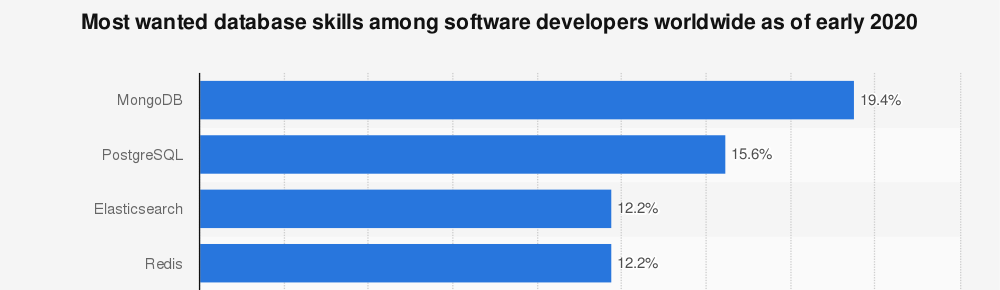
\includegraphics[width=1.0\linewidth]{img/statista_db.png}
	\caption{Stack Overflow. "Most wanted database skills among software developers worldwide as of early 2020." Chart. February 15, 2020. Statista. Accessed August 18, 2020. \url{https://www.statista.com/statistics/793854/worldwide-developer-survey-most-wanted-database/}}
\end{figure}

ElasticSearch erreicht eine sehr gute Suchperformance durch das Verwenden von Indizes und einer guten Tokenisation der indizierten Daten. Zusätzlich ist ElasticSearch so aufgebaut, dass es einfach innerhalb eines Clusters verwendet werden kann. Die in einem Cluster vorhandenen Nodes können auf verschiedenste Weisen konfiguriert werden. Innerhalb von ElasticSearch gibt es auch die Möglichkeit, \ac{ML} Funktionen zu verwenden. Diese \ac{ML} Funktionen sind die Grundlage für das Konzept, welches das Problem lösen könnte. Dazu werden, zusätzlich zu \ac{ML}-Nodes noch andere Produkte der Firma Elastic verwendet.

Ein weiteres Produkt nennt sich \ac{APM}\footnote{\url{https://www.elastic.co/de/apm}}, welches die Möglichkeit hat sowohl anwendungsspezifische Daten, als auch hardwarespezifische (oder containerspezifische) Metriken zu sammeln und direkt in einen entsprechenden ElasticSearch-Index zu speichern. Für das \ac{APM} gibt es Integrationen für alle wichtigen Programmiersprachen\footnote{\url{https://www.elastic.co/guide/en/apm/get-started/current/index.html}}. Diese Software liefert wichtige Informationen über den aktuellen Zustand eines Services und bietet auch gleichzeitig eine zentralisierte Sammelstelle für diese Metriken. 

Dies erfüllt die Punkte vier und fünf der Anforderung \vref{chap:Anforderungen}. Das initiale Aufsetzen der Infrastruktur benötigt allerdings durchaus produktspezifisches Know-How. Danach ist es aber ein sehr einfacher Prozess neue Services anzuschließen, da dies rein auf Serviceebene, also von den implementierenden Teams erledigt werden kann und unterstützt somit den dezentralen Ansatz einer Microservicearchitektur. Es fehlt allerdings noch die Auswertung und Aufbereitung der durch \ac{APM} gesammelten Daten. Dazu kann das Visualisierungstool von Elastic, \textbf{Kibana}\footnote{\url{https://www.elastic.co/de/kibana}}, verwendet werden. \\
Kibana nutzt die vorhandenen Indizes in einem ElasticSearch Cluster, um verschiedenste Operationen, meistens visualisierender Art, durchzuführen. Dort können auch eigene Visualisierungen konfiguriert werden, welche dem Endnutzer ermöglichen, eine für ihn optimale Informationslandschaft zu gestalten. Dies erfüllt das zweite definierte Kriterium aus \vref{chap:Anforderungen}, da es die durch \ac{APM} gesammelten Daten zu wertvollen Informationen aufbereitet, welche Hinweise geben auf den internen Zustand eines Services.

Die Kombination aus \ac{APM} und Kibana stellt also Tools dar, die einen Fokus auf die Observability haben. Das eigentliche Problem beinhaltet aber auch, dass ein Nutzer sehr schnell wissen muss, um welchen Fehler es sich handelt und wie groß die Auswirkungen sind. Zusätzlich ist es wichtig, bereits während der Entwicklung eines Services zu wissen, in welcher Umgebung sich der Service befindet. Um diese Governanceaspekte in diesen Lösungsvorschlag zu integrieren, kommen die bereits angesprochenen \ac{ML} Nodes ins Spiel. Diese bieten die Möglichkeit, eine Analyse der Daten in einem Index durchzuführen. Ab dann kann festgestellt werden, ob ein System \enquote{normal} operiert oder nicht. Sollten nun Metriken aus \ac{APM} in dem Index gespeichert werden, welche Hinweise auf einen Fehler enthalten, so wird die Analyse dies erkennen und es besteht die Möglichkeit des schnellen Entdeckens des Fehlers. Gleichzeitig beinhaltet die Nutzung der \ac{ML} Funktionalität auch einige Schwierigkeiten.

So ist es z.B. während der Analyse schwer zu unterscheiden, ob eine erkannte Anomalie wirklich ein Fehler ist oder einfach nur ein neuer Service, der hinzugefügt wurde. Es ist auch nur schwer möglich die Metriken unterschiedlicher Services in einer einzelnen \ac{ML} Node auszuwerten, da durch unterschiedliche Hardwaredaten der verschiedenen Services ein sehr breites Spektrum als \enquote{normal} angesehen wird. Es gilt also hierfür eine Lösung zu finden, welche nicht beinhaltet, dass für jeden neuen Service eine neue \ac{ML} Pipeline angelegt werden muss.

Die Idee dieses bestehenden Tools zu verwenden, um das Problem zu lösen ist prinzipiell nicht von der Hand zu weisen, da auch einige wesentliche Anforderungen aus \vref{chap:Anforderungen} erfüllt werden. Allerdings bringt es auch Schwierigkeiten mit sich, die es vor der Einführung und dauerhaften Nutzung dieser Tools zu lösen gilt.

\section{Konzept unter Nutzung einer Graphdatenbank}

Im ersten Abschnitt dieses Kapitels wurden bereits Grundlagen im Bezug auf Graphen und deren Eigenschaften erläutert. Die Idee Graphen zu verwenden, um Abhängigkeiten und Verbindungen zwischen Elementen darzustellen, ist nicht neu \autocite{Ren2018}. Bereits \citeyear{Metayer1998} erläuterte \citeauthor{Metayer1998} in \textit{\citetitle{Metayer1998}} einen Ansatz, wie man mithilfe formaler Sprachen die Softwarearchitektur in einem Graphen abbilden kann \autocite{Metayer1998}.

\begin{example}[Abhängigkeitsgraphen]
	Abhängigkeitsgraphen werden auch in Toolings für verschiedene Programmiersprachen verwendet. Ein Beispiel ist JavaScript. Diese ermöglichen es Dateien verschiedenen Formats miteinander zu kombinieren und in einer Datei, dem Bundle, zusammenzuführen. Dabei ist es wichtig, dass alle Dateien in der richtigen Reihenfolge in das Bundle integriert werden, um am Ende ein lauffähiges Programm zu erhalten. Um zu wissen, welche Dateien in welcher Reihenfolge eingefügt werden müssen, wird ein Abhängigkeitsgraph erstellt, an dem abgelesen werden kann, welche Datei benötigt wird, um eine andere valide Datei zu erhalten.
\end{example}

Das Konzept eines Abhängigkeitsgraphen ist auch die Grundlage für die Idee, die Abhängigkeiten zwischen Services über einen Graphen darzustellen. Für die Realisierung des Konzeptes kann eine beliebige Graphdatenbank gewählt werden. Dabei sollte aber darauf geachtet werden, dass es sich um eine \enquote{native} Graphdatenbank handelt. Das bedeutet, dass der primäre Anwendungsfall des \ac{DBMS} die Darstellung und Speicherung der Daten in einem Graphen ist. Andere \ac{DBMS}, wie z.B. Elastic oder MongoDb bieten auch die Möglichkeit Daten mithilfe von Graphen darzustellen und zu speichern. In diesen Datenbanken sind die Graphen nur unter Zuhilfenahme einer großen Anzahl an Indizes realisierbar \autocite{JoyChao2016}. Diese \enquote{nicht-nativen} Graphen haben oftmals eine deutlich schlechtere Performance als ein \ac{DBMS}, welches einen nativen Graphen realisiert.\\
Für den oben beschriebenen Anwendungsfall sollte also ein \ac{DBMS} gewählt werden, welche eine native Implementierung eines Graphen besitzt.

\subsection{Das Konzept einer graphbasierten Service-Registry}

Wie bereits in Beispiel \vref{exp:microserviceGraph} beschrieben, kann die Menge der Knoten in einem Graphen mit den Microservices innerhalb eines Unternehmens gleichgesetzt werden. Diese Knoten können mithilfe einer Graphdatenbank noch zusätzliche Eigenschaften erhalten. Im folgenden wird exemplarisch \textbf{Neo4j}\footnote{\url{https://neo4j.com/}} als Repräsentant eines graphbasierten \ac{DBMS} verwendet. Allerdings sind die genutzten Funktionen auch in anderen Graphdatenbanken verfügbar.

Die grundlegende Idee soll anhand eines sehr einfachen Graphen beschrieben werden. Dieser Graph $G$ ist definiert mit:
\begin{itemize}
	\item $V = \{\text{Service A, Service B}\}$ und
	\item $A = \{(\text{Service A},\text{Service B}), (\text{Service B}, \text{Service A})\}$
\end{itemize}

Diese Definition führt zu folgenden Graphen:

\begin{figure}[h]
	\centering
	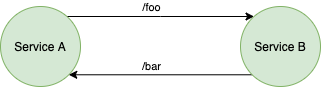
\includegraphics[width=0.65\linewidth]{img/service_dependencies.png}
	\caption[Abbildung eines simplen Abhängigkeitsgraphen]{Visualisierung des Graphen\\Quelle: Eigen}
\end{figure}

Da es sich um einen gerichteten Graphen mit geordneten Tupeln als Elemente der Kantenmenge $V$ handelt, kann die Richtung der Abhängigkeit erkannt werden. Zu lesen ist es folgendermaßen:

\begin{center}
	Service A benötigt den \texttt{/foo}-Endpunkt von Service B\\
	Service B benötigt den \texttt{/bar}-Endpunkt von Service A
\end{center}

In der mathematischen Darstellung alleine ist allerdings noch keine Information bzgl. der Abhängigkeit zu erkennen. In einem \ac{DBMS} wie Neo4j ist dies allerdings möglich, da es dort möglich ist sowohl an Knoten (Nodes), als auch an Kanten (Relations) Schlüssel-Wert-Paare zu speichern \footnote{\url{https://neo4j.com/developer/graph-database\#property-graph}}. Dies ermöglicht einer Service-Registry die benötigten Metadaten zu speichern, sowohl um die Services an den Knoten, als auch um die Abhängigkeiten näher zu beschreiben.

\subsection{Mögliche Realiserungen des Konzepts}

Im Folgenden werden verschiedene Ansätze präsentiert, welche versuchen, die durch das Datenmodell geschaffenen Möglichkeiten, so umzusetzen, dass eine den in \vref{chap:Anforderungen} beschriebenen Anforderungen entspricht.\\ Um eine den Anforderungen gerechte Service-Registry entwickeln zu können, werden zwei Komponenten benötigt. Zum einen, auch der Kernbestandteil, wird eine \textit{zentrale Komponente} benötigt, die Funktionen einer Service-Registry realisiert. Das bedeutet, sie muss alle Services kennen und auch deren Beziehung zueinander darstellen. Es stellt sich nun die Frage, wie die Informationen über Art und Zusammenhang der Services zu der zentralen Komponente gelangen. Dazu werden zwei Verfahren vorgestellt:

\subsubsection*{1. Statischer Ansatz}
Wie bereits in der Definition eines Microservice festgehalten, ist es die Pflicht des dafür zuständigen Teams parallel zum Service auch eine \textbf{Service Defintion} bereitzustellen. Dafür können die schnittstellenspezifischen Standards genutzt werden. Ein offener Standard zum Beschreiben von REST Schnittstellen ist OpenAPI 3.0\footnote{\url{https://swagger.io/specification/}}. REST oder RESTful Services sind die aktuell meistgenutzen Formate bei Webservices. Innerhalb dieses Standards gibt es außerdem die Möglichkeit, weitere Metadaten zum Beschreiben eines Services zu speichern. Um dem Graphen die benötigten Daten bereitzustellen, kann das für einen Service zuständige Team die Abhängigkeiten in ein speziell definiertes Metadatenfeld eintragen\footnote{\url{https://swagger.io/docs/specification/openapi-extensions/}}. Die zentrale Komponente, die dafür verantwortlich ist den Graphen aufzubauen, könnte dann auf Basis dieser Informationen einen die Architektur repräsentierenden Graphen konstruieren. 

Dabei wird für jede eingelesene Service-Defintion ein neuer Knoten im Graphen angelegt. Es kann dann auf Basis von eigenen Identifiern oder von den angegebenen URL's bei den Abhängigkeiten eine Kante zwischen dem neu erstellten Service und der Abhängigkeit erstellt werden.

% TODO: Evtl. noch den Algorithmus zum auslesen und konstruieren eines Graphen reinhauen oder ein Bild von nem neo4j graphen der sowas repräsentiert

Diese Methode bringt allerdings einige Probleme mit sich, welche die Nutzung einer solchen Service-Registry erschweren würden:

\begin{enumerate}
	\item Durch den statischen Ansatz besteht die Notwendigkeit, Informationen über den eigenen Service, sowie über dessen Abhängigkeiten manuell in einem Dokument zu hinterlegen. Dies erhöht das Fehlerpotenzial immens, da sehr viele nicht automatisierte Schritte durchgeführt werden müssen. Zusätzlich müssen die Abhängigkeiten, sollten diese sich ändern, manuell in dem Dokument angepasst werden.
	\item Desweiteren stellt sich die Frage, woran ein Service identifiziert werden kann. In dem Beispiel wurde mithilfe eines extra Feldes \texttt{x-service-identifier} versucht, eine eindeutige Identifizierbarkeit zu gewährleisten. Diese Methode hat allerdings mehrere Schwachstellen. Es muss entweder vor einem Servicedeployment sichergestellt werden, dass die Service-ID einzigartig im zu untersuchenden Bereich ist oder das Deployment muss von der Service-Registry verhindert werden, solange bis ein einzigartiger Identifier gewählt wurde. Beide Varianten sind nicht nutzerfreundlich und mit einem zu hohen Aufwand verknüpft.
	\item Die beiden vorherigen Probleme führen dazu, dass das Deployment eines Services nun nicht mehr einfach und im Rahmen einer agilen Entwicklung erfolgen kann, da nun ein sehr hoher administrativer Aufwand damit verbunden ist. Auch kann eine Aktualisierung des Graphen, der als Repräsentant der Service-Registry dient, nur dann erreicht werden, wenn eine neue Version der Service-Definition vorhanden ist. Dieser Ansatz widerspricht der eigentlichen Anforderung, das Fehlerrisiko so gering wie möglich zu halten.
	\item Es ist außerdem nicht möglich zu erkennen, wie stark die Abhängigkeit ist. Das bedeutet, bricht der Service komplett zusammen, da es eine notwendige Abhängigkeit ist, die sehr oft genutzt wird oder besteht eher ein geringeres Risiko, da die Verbindungen nur sehr selten genutzt wird.
\end{enumerate}

\subsubsection*{2. Dynamischer Ansatz}

Aus den Problemen der statischen Methode lässt sich erkennen, dass viele Prozesse automatisiert ablaufen müssen. Zusätzlich dazu fehlen noch wichtige Bestandteile einer Service-Registry. Dazu zählen unter anderem:

\begin{enumerate}
	\item die Service-Discovery,
	\item das automatische Hinzufügen und Aktualisieren in dem Graphen und
	\item die Einführung einer Gewichtung, um zu erkennen wie \enquote{stark} eine Abhängigkeit zwischen zwei Services ist.
\end{enumerate}

Die Lösung für die in Punkt eins und zwei beschriebenen Probleme lässt sich mithilfe einer Prozessautomatisierung erreichen. Dazu wird der vorherige Ansatz des manuellen Eintragens der Serviceinformationen in die Servie-Defintion ersetzt durch die Idee einer automatischen Service-Anmeldung. Mithilfe eines Plugins für die in dem Microservice verwendete Servertechnologie kann während des Startvorgangs eine Anmeldung an der zentralen Komponente der Service-Registry durchgeführt werden. Diese Anmeldung mithilfe des folgenden Ablaufs beschrieben werden:

\begin{figure}[h]
	\centering
	
	\caption{TODO: Protocoll aufmalen}
\end{figure}

\begin{enumerate}
	\item Während des Hochfahrens des Services meldet sich der \enquote{Client} bei der zentralen Komponente als Service an. Die zentrale Komponente kann dann dem Service einen Service-Identifier zuweisen, der zur späteren Identifiezierung sowohl in der Registry selbst, als auch bei anderen Tools dienen kann.
	\item Im nächsten Schritt wird dann von dem Service ein Endpunkt (entweder vordefiniert durch die Registry oder ausgehandelt während des initialen Verbindungsaufbaus) bereitgestellt, der Informationen über die Aktivität seit der letzten Abfrage dieses Endpunktes enthält. Dabei kommt es vor allem darauf an, welche anderen Services angefragt werden. Jeder Service sollte einen eigenen Header mitsenden, der den von der Registry bereitgestellten Identifier beinhaltet. So kann später in der zentralen Komponente der Registry festgestellt werden, welche Services zur Bearbeitung der eigenen Anfrage, Informationen aus anderen Services benötigen.
	\item Im letzten Schritt wird innerhalb der zentralen Komponenten die Abfrage dieses Endpunktes in regelmäßigen Intervallen verwaltet.
\end{enumerate}

In einer Client-Bibliothek müssen also nur Funktionen zum Austausch über einen Identifier und Sammeln von Requestinformationen implementiert werden. Dies hat den Vorteil, dass die Client-Bibliotheken sehr klein gehalten werden können und auch nur eine geringe Runtime-Cost einführen, somit sehr wenige Performanceeinbußen mit der Nutzung einer solchen Registry einhergehen.

\subsection{Die zentrale Komponente}

Im folgenden Abschnitt soll nun kurz auf die Funktionalität innerhalb der zentralen Komponente eingegangen werden. Im speziellen wird dabei dargestellt, wie der Graph auf Basis der gesammelten Nutzungsdaten aufgebaut werden kann. Die Methode, wie der Graph erstellt wird soll zunächst mathematisch begründet werden. Danach wird ein Implementierungsvorschlag erläutert.

Dazu wird zunächst die Defintion eines Flussnetzwerks \vref{def:Fluss} wieder aufgegriffen. Ein Flussnetzwerk wird deshalb gewählt, da die Abhängigkeiten zwischen den Services gewichtet werden auf Basis von deren Nutzung. Es müssen also zwei Funktionen bereitgestellt werden, eine Kapazitätsfunktion $c$ und eine Flussfunktion $f$.

Die Abbildung $f: A \rightarrow \mathbb{R_+}$ wird folgendermaßen definiert:

\begin{equation*}
	f(a) = \sum (\text{Request von } a_1 \text{ nach } a_2) \text{, mit } a = (a_1, a_2) \in A
\end{equation*}

Mithilfe dieser Funktion kann jeder Kante im Graphen ein postiver ganzzahliger Wert zugewiesen werden. Nun muss noch eine Kapazitätsfunktion $c: V \times V \rightarrow \mathbb{R_+}$ definiert werden, damit ein vollständiges Flussnetzwerk vorliegt. Dafür wird folgendende Methode gewählt:

\begin{equation*}
	c(v_1,v_2) = \begin{cases}
		f((v_1,v_2)) \text{, wenn } (v_1,v_2) \in A\\
		0 \text{ sonst } \\
	\end{cases}
\end{equation*}

Das bedeutet also, jede Kante besitzt nun eine Gewichtung. Diese Gewichtung ist abhängig von der tatsächlich registrierten Nutzung der Verbindung zwischen zwei Services. Dieses mathematische Konzept kann nun mithilfe von Neo4j umgesetzt werden. Die hier Werte der Gewichtungsfunktion $f$ werden als Wert an der \textit{Relation} zwischen den entsprechenden \textit{Nodes} gespeichert. Die Gewichtungsfunktion $f$ ist allerdings von der Anzahl der Anfragen zwischen zwei Services abhängig. Diese Anzahl wird von der dezentralen Komponente gesammelt. 

Beispielsweise könnte mithilfe dieser Komponente ein Endpunkt an jedem Service registriert werden, der auf Anfrage eine Antwort in JSON-Format bereitstellt, die folgendermaßen aufgebaut sein könnte:

\begin{lstlisting}[language=json, caption={Antwort über Nutzung anderer Services}]
{
	"service-identifier": {
		"Endpunkt": "Anzahl",
		// ..
	},
	// ...
}
\end{lstlisting}

\section{Bewertung und Gegenüberstellung der Methoden}

\begin{itemize}
	\item Kurze Einführung in Graphdatenbanken, im speziellen Neo4j. Wieso passen die so gut? referenzieren auf Bilder und \enquote{Abhängigkeiten} Wie kann damit eine Lösung konstruiert werden?
	\begin{itemize}
		\item Statischer Ansatz $\Rightarrow$ von den Entwicklern definierte Abhängigkeiten werden in der Service-Definition angegeben. Der Graph kann aus diesen SD's erstellt werden. Hier gibt es Probleme: Manuelle Veranwtortlichkeit widerspricht eigentlicher Idee von Risikoeinschätzung, da ein neuer Fehler Mensch eingebaut wird.
		\item Automatischer nutzungsbasierter, somit dynamischer Aufbau des Graphen. Prinzip ähnlich wie bei Prometheus (populäres Tool zum sammeln von Metriken). Konzept ähnlich wie Distributed Tracing. Dort werden alle Traces mit ihren Spans zusammengefasst und zentral ausgewertet. Kombination aus dieser Idee mit Prometheus-Ansatz sieht dann folgendermaßen aus:
		
		Jeder Service exposed einen \texttt{/traffic}-Endpoint, der unstrukturierte Daten bzgl. der Netzwerkaktivität enthält. Diese können dann in einem Service, der für den Aufbau des Graphen zuständig ist, zu eben diesem umgewandelt werden.
		\item Es kann zusätzlich überlegt werden, ob anstatt dieses \texttt{PULL}-Verfahrens eine Push-Variante gewählt wird, welche ähnlich wie \texttt{fluentd} als Sidecar in einer containererisierten Umgebung läuft. Die könnte dann periodisch die Netzwerkdaten pushen, wenn sie Zugriff darauf hat.
	\end{itemize}
	\item Es kann überlegt werden welche Metadaten zusätzlich im Rahmen dieses Graphen eine sinnvolle Ergänzung bieten würden, sodass ein weiterer Mehrwert geschaffen werden kann. (Ist das noch im Rahmen der Arbeit? Kommt das eher in den Ausblick mit ein paar Ideen?)
	\item Wie können jetzt die Sachen in dem coolen Graphen genutzt werden?
	\begin{itemize}
		\item Kurze \texttt{CYPHER-QUERIES} Aufschreiben:
		\begin{itemize}
			\item Wie finde ich affectete services raus
			\item was passiert wenn ein Service X ausfällt
			\item Was ist die Zentralste Komponente in meinem Unternehmen
			\item usw.
		\end{itemize}
	\end{itemize}
\end{itemize}
